\subsection{Federated Software Architecture}
\begin{frame}{Recap: Conways Law}
	\begin{fancycolumns}[animation=none]
		\nextcolumn
		\vspace{-8mm}
		\href{https://twitter.com/conways_law}{\pic[width=\linewidth,trim=0 50 0 0,clip]{people/melvin-conway}}
		\vspace{-7mm}
		
		\begin{note}{Melvin E. Conway (1968) \mysource{\href{http://www.melconway.com/Home/Committees_Paper.html}{melconway.com}}}
			\mycite{Any organization that designs a system [...] will produce a design whose structure is a copy of the organization's communication structure.}
		\end{note}
	\end{fancycolumns}
\end{frame}

\begin{frame}{\insertsubsection\ \mytitlesource{\staron}}
	\begin{fancycolumns}[columns=3,widths={5,90,5},animation=none]
		\nextcolumn
		\myexampletight{}{\centering\pic[width=\linewidth]{automotive/federated_architecture}}
		\nextcolumn
	\end{fancycolumns}
\end{frame}

\begin{frame}{\insertsubsection\ \mytitlesource{\vdovic}}
	\mydefinition{Bus Systems for Automotive Systems}{
		\small \centering
		\begin{tabular}{
				>{\columncolor[HTML]{EFEFEF}}l |l|l|l|l}
			\textbf{Bus System}       & \cellcolor[HTML]{EFEFEF}\textbf{CAN}           & \cellcolor[HTML]{EFEFEF}\textbf{FlexRay} & \cellcolor[HTML]{EFEFEF}\textbf{LIN} & \cellcolor[HTML]{EFEFEF}\textbf{MOST} \\ \hline
			\textbf{Type}             & event-triggered                                & time-triggered                           & subbus                               & multimedia                            \\ \hline
			\textbf{Application}      & \makecell[lc]{ABS, battery management \\ system, engine control} & \makecell[lc]{drive-by-wire \\ systems}                   & \makecell[lc]{door locking, \\ powered windows}        & \makecell[lc]{entertainment, \\ navigation}             \\ \hline
			\textbf{Bandwidth}        & up to 1 Mbit/s                                 & up to 10 Mbit/s                          & up to 20 kbit/s                      & up to 24.8 Mbit/s                     \\ \hline
			\textbf{Access Control}   & CMSA/CD                                        & TDMA                                     & Polling                              & TDM, CMSA/CA                          \\ \hline
			\textbf{Error protection} & CRC, parity bits                               & CRC, bus guardian                        & checksum, parity bits                & \makecell[lc]{CRC, checksum, \\ parity bits}           
		\end{tabular}
		
	}
\end{frame}

\xkcdframe{2212}

\subsection{Centralized Software Architecture}
\begin{frame}{\insertsubsection\ \mytitlesource{\staron}}
	\begin{fancycolumns}[columns=3,widths={5,90,5},animation=none]
		\nextcolumn
		\myexampletight{}{\centering\pic[width=\linewidth]{automotive/centralized_architecture}}
		\uncover<2->{\mynote{}{redundancy still needed for the fail safe mode}}
		\nextcolumn
	\end{fancycolumns}
\end{frame}

\begin{frame}{\insertsubsection\ \mytitlesource{\vdovic}}
	\myexampletight{Bus Systems in Use}{
		\centering \footnotesize
%		\begin{tabular}{
%				>{\columncolor[HTML]{EFEFEF}}l 
%				>{\columncolor[HTML]{EFEFEF}}l |l|l|l}
%			\multicolumn{2}{l|}{\cellcolor[HTML]{EFEFEF}}                                                            & \cellcolor[HTML]{EFEFEF}\textbf{2018 Nissan Leaf}                       & \cellcolor[HTML]{EFEFEF}\textbf{2018 Checrolet Bolt}               & \cellcolor[HTML]{EFEFEF}\textbf{Tesla Model S P100D} \\ \hline
%			\multicolumn{2}{l|}{\cellcolor[HTML]{EFEFEF}\textbf{Price}}                                              & \$29,990                                                                & \$36,620                                                           & \$135,000                                            \\ \hline
%			\multicolumn{1}{l|}{\cellcolor[HTML]{EFEFEF}}                                        & \textbf{Number of ECUs}                & 3 - 8                                                                   & 3 - 8                                                              & 3 - 4                                                \\ \cline{2-5}
%			\multicolumn{1}{l|}{\cellcolor[HTML]{EFEFEF}}                                       & \textbf{Bus Systems}                   & \makecell[lc]{multiple CAN buses, \\ multiple LIN buses, \\ FlexRay }                        & \makecell[lc]{multiple CAN buses, \\ multiple LIN buses, \\ FlexRay }                   & \makecell[lc]{multiple CAN buses, \\ multiple LIN buses, \\ Ethernet}     \\ \cline{2-5}
%			\multicolumn{1}{l|}{\cellcolor[HTML]{EFEFEF}}                                         & \textbf{\makecell[lc]{Infotainment \\ Panel}}            & \makecell[lc]{vehicle information display, \\ 7-inch touchscreen}                         & \makecell[lc]{8-inch driver information center, \\ 10.2-inch touchscreen }           & \makecell[lc]{driver display, \\ 17-inch touchscreen }                 \\ \cline{2-5}
%			\multicolumn{1}{l|}{\multirow{-4}{*}{\cellcolor[HTML]{EFEFEF}\textbf{Softwarized}}} & \makecell[lc]{\textbf{Infotainment \\ Operating System}} & \makecell[lc]{Windows Embedded Automotive, \\ support for Android Auto \\ and Apple CarPlay } & \makecell[lc]{MyLink based on QNX OS, \\ support for Android Auto \\ and Apple CarPlay} & \makecell[lc]{ modified version of \\ Ubuntu Linux }                   
%		\end{tabular}

	\begin{tabular}{
			>{\columncolor[HTML]{EFEFEF}}l 
			>{\columncolor[HTML]{EFEFEF}}l |l|l|l}
		\multicolumn{2}{l|}{\cellcolor[HTML]{EFEFEF}}                                                                                & \cellcolor[HTML]{EFEFEF}\textbf{2018 Nissan Leaf}                       & \cellcolor[HTML]{EFEFEF}\textbf{2018 Checrolet Bolt}               & \cellcolor[HTML]{EFEFEF}\textbf{Tesla Model S P100D} \\ \hline
		\multicolumn{2}{l|}{\cellcolor[HTML]{EFEFEF}\textbf{Price}}                                                                  & \$29,990                                                                & \$36,620                                                           & \$135,000                                            \\ \hline
		\multicolumn{1}{l|}{\cellcolor[HTML]{EFEFEF}}                                       & \textbf{Number of ECUs}                & 3 - 8                                                                   & 3 - 8                                                              & 3 - 4                                                \\ \cline{2-5} 
		\multicolumn{1}{l|}{\cellcolor[HTML]{EFEFEF}}                                       & \textbf{Bus Systems}                   & \makecell[lc]{multiple CAN buses, \\ multiple LIN buses, \\ FlexRay}                         & \makecell[lc]{multiple CAN buses, \\ multiple LIN buses, \\ FlexRay}                    & \makecell[lc]{multiple CAN buses, \\ multiple LIN buses, \\ Ethernet}     \\ \cline{2-5} 
		\multicolumn{1}{l|}{\cellcolor[HTML]{EFEFEF}}                                       & \bfseries\makecell[lc]{ Infotainment \\ Panel}            & \makecell[lc]{vehicle information display, \\ 7-inch touchscreen}                         & \makecell[lc]{8-inch driver information center, \\ 10.2-inch touchscreen  }          & \makecell[lc]{ driver display, \\ 17-inch touchscreen }                 \\ \cline{2-5} 
		\multicolumn{1}{l|}{\multirow{-4}{*}{\cellcolor[HTML]{EFEFEF}\textbf{Softwarized}}} & \bfseries\makecell[lc]{ Infotainment \\ Operating System } & \makecell[lc]{Windows Embedded Automotive, \\ support for Android Auto \\ and Apple CarPlay} & \makecell[lc]{MyLink based on QNX OS, \\ support for Android Auto \\ and Apple CarPlay} & \makecell[lc]{modified version of \\ Ubuntu Linux }                   
	\end{tabular}

	}
\end{frame}

\subsection{AUTOSAR: Standardization of Software Architectures}
\begin{frame}{\insertsubsection\ \mytitlesource{\staron}}
	\begin{fancycolumns}
		\begin{note}{Motivation}
			\begin{itemize}
				\item more efficient collaboration between different OEMs and tiers \deutsch{Automobilhersteller und Zulieferer}
				\item easier exchange of hardware
				\item common components
				\item common operating system
			\end{itemize}
		\end{note}
		\nextcolumn
		\begin{definition}{AUTOSAR}
			\begin{itemize}
				\item \emph{ATU}omotive \emph{O}pen \emph{S}ystem \emph{AR}chitecture
				\item reference architecture + development methodology + AUTOSAR platform
				\item \emph{AUTOSAR Classic Platform}\\ for traditional mechatronic systems (e.g., doors, air conditioning)
				\item \emph{AUTOSAR Adaptive Platform}\\ for modern system (e.g., autonomous driving, connectivity)
			\end{itemize}
		\end{definition}
	\end{fancycolumns}
\end{frame}

\subsection{Example Architecture of a Modern Car}
\begin{frame}[b]{\insertsubsection\ \mytitlesource{\vdovic}}
	\begin{fancycolumns}[columns=3,widths={5,80,5},animation=none]
		\nextcolumn
		\vdoviclink{\pic[width=\linewidth,page=7,trim=55 395 60 75,clip]{automotive/VBP-Access19}}
		\nextcolumn
	\end{fancycolumns}
\end{frame}

%\subsection{Forschung zu Automotive Software Engineering}
%\begin{frame}{\insertsubsection\ \mytitlesource{\asesurvey}}
%	\begin{fancycolumns}[widths={60}]
	%		\asesurveylink{\includegraphics[width=\linewidth,page=12,trim=35 410 35 60,clip]{HBP+-JSS17}}
	%	\nextcolumn
	%		\asesurveylink{\includegraphics[width=\linewidth,page=12,trim=320 165 35 420,clip]{HBP+-JSS17}}
	%	\end{fancycolumns}
%\end{frame}

\subsection{Architectural Patterns in Automotive Software}
\begin{frame}{Recap: Architectural Patterns\ \deutsch{Architekturmuster}}
	\slideArchitecturalPattern
\end{frame}

\subsubsection{Layered Architecture}
\begin{frame}{\insertsubsubsection\ \mytitlesource{\staron}}
		\myexampletight{Reference Architecture for Autonomous Driving}{\centering\pic[width=.65\linewidth]{automotive/layered_architecture}}
\end{frame}

\subsubsection{Pipe-and-Filter Architecture}
\begin{frame}{\insertsubsubsection\ \mytitlesource{\staron}}
		\myexampletight{Image Processing}{\centering\pic[width=\linewidth]{automotive/pipe_filter_architecture}}
\end{frame}

%\subsubsection{Client-Server Architecture}
%\begin{frame}{\insertsubsubsection\ \mytitlesource{\staron}}
%	\begin{fancycolumns}[columns=3,widths={5,66,5},animation=none]
%		\nextcolumn
%		\myexampletight{Fleet Management \deutsch{Flottenmanagement}}{\centering\staronlink{\pic[width=\linewidth,page=60,trim=75 265 85 245,clip]{automotive/S21}}}
%		\mynote{}{Telematics = Telecommunication + Informatics}
%		\nextcolumn
%	\end{fancycolumns}
%\end{frame}

\subsubsection{Publisher-Subscriber Architecture}
\begin{frame}{\insertsubsubsection\ \mytitlesource{\staron}}
		
		\myexampletight{Speed Control}{\centering\pic[width=.8\linewidth]{automotive/publish_subscribe_architecture}}
		\mynote{Publisher-Subscriber Architecture}{similar to observer pattern but on architectural level}
	
\end{frame}

\begin{frame}[b]{Recap: Gordon Bell}
	\begin{fancycolumns}[animation=none]
		\nextcolumn
		\vspace{-15mm}
		\href{https://en.wikipedia.org/wiki/File:Gordon_Bell.jpg}{\pic[width=\linewidth,trim=175 0 0 0,clip]{people/gordon-bell}}
		\vspace{-7mm}
		
		\begin{note}{Gordon Bell \mysource{\href{https://dl.acm.org/doi/10.1145/1968.381154}{Bentley 1984}}}
			\mycite{The cheapest, fastest, and most reliable components are those that aren’t there.}
		\end{note}
	\end{fancycolumns}
\end{frame}

